%\documentclass{article}
\documentclass{www2010-submission}
\usepackage{times}
%\usepackage{uist}
\usepackage{url}
\usepackage{graphics}
\usepackage{color}
%
%\newcommand{\want}[1]{{[\color{blue} WANT: #1]}}
%\newcommand{\todo}[1]{{[\color{blue} TODO: #1]}}
%\newcommand{\idea}[1]{{[\color{blue} IDEA: #1]}}
%\newcommand{\node}[1]{{[\color{blue} NOTE: #1]}}

\newcommand{\want}[1]{}
\newcommand{\todo}[1]{}
\newcommand{\idea}[1]{}
\newcommand{\node}[1]{}


\begin{document}

\toappear

\bibliographystyle{plain}

\title{Highlighting Disputed Information on the Web}

%%
%% Note on formatting authors at different institutions, as shown below:
%% Change width arg (currently 7cm) to parbox commands as needed to
%% accommodate widest lines, taking care not to overflow the 17.8cm line width.
%% Add or delete parboxes for additional authors at different institutions. 
%% If additional authors won't fit in one row, you can add a "\\"  at the
%% end of a parbox's closing "}" to have the next parbox start a new row.
%% Be sure NOT to put any blank lines between parbox commands!
%%

\numberofauthors{5}

\author{
	Author list to be determined
}

%\author{
%\alignauthor Rob Ennals\\
%       \affaddr{Intel Labs Berkeley}\\
%       \affaddr{2150 Shattuck Ave}\\
%       \affaddr{Berkeley, CA, USA}\\
%       \email{robert.ennals@intel.com}
%\alignauthor Beth Trushkowsky\\
%       \affaddr{Computer Science Division}\\
%       \affaddr{University of California at Berkeley}\\
%       \affaddr{Berkeley, CA, USA}\\
%       \email{trush@berkeley.edu}
%\alignauthor John Mark Agosta\\
%       \affaddr{Intel Labs Santa Clara}\\
%       \affaddr{2200 Mission College Blvd}\\
%       \affaddr{Santa Clara, CA, USA}\\
%       \email{john.m.agosta@intel.com}
%}
%
%\additionalauthors{Additional authors: Tad Hirsch (Intel Research PaPR, email: {\texttt{tad.hirsch@intel.com}}) and Tye Rattenbury (Intel Research PaPR), email: {\texttt{tye.rattenbury@intel.com}})}


\maketitle

%RULE: Don't cite media reports unless I have to - some reviewers don't like it


\abstract

We describe Dispute Finder, a browser extension that helps a user know when information they read online is disputed -- where by 'disputed' we mean that a source that they might trust expresses a different point of view.  As a user browses the web, Dispute Finder examines the text on pages that the user is browsing and highlights any phrases that appear to be supporting claims from its database of known disputed claims. If a user clicks on a highlighted phrase, Dispute Finder will show the user a summary of arguments from other sources that support other points of view.

Disputed Claims can be submitted by users, or may be found automatically by crawling web sites that already maintain lists of disputed claims. Dispute Finder identifies instances of disputed claims by running a simple textual entailment algorithm inside the browser extension, referring to a cached local copy of a subset of our claim database.

Performing these tasks well is a hard problem, and we do not yet claim to have an implementation that is good enough to be compelling for most users. We do however believe that Dispute Finder attacks an interesting problem that, if addressed well, could significantly improve the utility of the web.


\category{H.4.m}{Information Systems}{Miscellaneous}
\category{H.4.2}{Information Systems}{Decision Support}
\category{H.5.2}{User Interfaces}{Graphical User Interfaces}

\terms{Design, Human Factors}

\keywords{Sensemaking, Annotation, Argumentation, Web, CSCW}


\tolerance=400 
  % makes some lines with lots of white space, but 	
  % tends to prevent words from sticking out in the margin

\section{INTRODUCTION}

\todo{update screenshots}

The web contains a huge amount of information, but some of this information is factually incorrect~\cite{Neumann2003,Resnik1998,Zhou2004} and some sites present only one side of a contentious issue~\cite{Herman2002}. 
If a user is to gain a broad understanding of a topic then they will need to either spend time looking for alternative points of view, or restrict themselves to sources that they believe they can trust to provide accurate and balanced information.
Even if a user tries to be careful, they can still be caught out by claims that they had not realized were disputed.
\todo{word this better}\todo{update all screenshots}

In this paper we describe Dispute Finder, a service that informs a user when information they read online is disputed by a source that they might trust. Our hope is that Dispute Finder will make it easier for a user to gain a broad view of a topic that they are interested in.

If a user has installed the Dispute Finder browser extension then it will highlight snippets of text on the web that make claims that Dispute Finder believes are disputed (Figure~\ref{highlight}). 
When a user clicks on a highlighted snippet, Dispute Finder will present a list of articles that present alternative points of view, each of which is from a source we believe the user is likely to trust (Figure~\ref{claimview}). 

Dispute Finder consists of a database, an API, and a firefox browser extension. The database contains information about the disputed claims that are known to be made on web sites, and hints about how to tell when a web page is making such a claim. The API allows an external client to determine whether particular content is making a disputed cliam. The firefox extension uses the API to determine whether the web pages a user browses make disputed claims. The API could also be used by other services that present users with potentially-disputed content, such as search engines, news readers, email programs, or content management systems.

\begin{figure}[tb]
	\begin{center}
	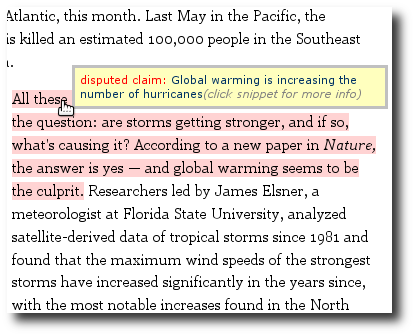
\includegraphics[width=6cm]{../screenshots/v2_highlight_shadow.png}
	\caption{Dispute Finder highlights snippets that make disputed claims}
	\label{highlight}
	\end{center}
\end{figure}

\begin{figure}[tb]
	\begin{center}
	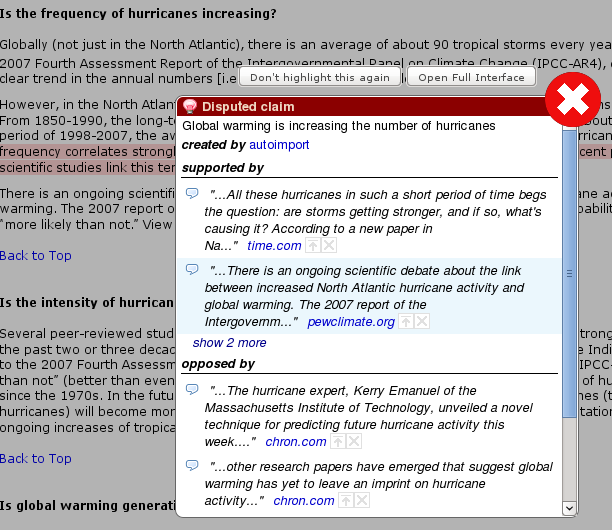
\includegraphics[width=8cm]{../screenshots/v2_popup_dim2.png}
	\caption{Click on a snippet to investigate evidence for the claim it makes}
	\label{claimview}
	\end{center}
\end{figure}

There are several design decisions that must be made when building a system such as this, which we will address in the remainder of the paper. In particular:

\begin{description}
\item[What claims are disputed?] In order to highlight claims as being disputed, we need to know what claims these are. To be useful, the set of known disputed claims needs to be both large (so people see some benefit) and accurate (so that people don't get annoyed by things that aren't actually disputed. We currently use a combination of crowdsourcing from users, and mining web sites such as Snopes and Politifact that already maintain lists of disputed claims. There are also other interesting alternative approaches that may be worth exploring. 

\item[What disputed claims should we tell the user about?] In some sense almost everything is disputed by someone. If we highlighted everything that was disputed by anyone then the tool would be too noisy to be useful. The challenge is to determine when the other point of view is something the user might take seriously. We do not yet have a large enough database of disputed claims for this to be a serious problem, but we believe that there may be interesting solutions.

\item[How do we tell that a snippet is making a disputed claim?] If a user is reading a web page that might contain disputed claims, then how do we determine which sentences are making disputed claims? We have experimented with several different approaches, each of which has different advantages and disadvantages. One can ask users to mark snippets individually. One can build a search tool that allows a user to find and mark similar snippets in bulk. One can provide an interface that allows a user to train a machine learning classifier to recognize snippets. One can use a textual entailment algorithm to recognize phrases that seem to have a similar meaning to the claim. We found advantages and disadvantages of all these approaches.

\item[How do we add highlights to the pages a user browses?] If a user is reading web pages, how should we augment that experience with information about disputed claims? Using a browser extension allows us to examine all content the user browses, but limits us to users who are prepared to install a browser extension~\cite{nolike-extension?}. Using a proxy~\cite{proxy?} has similar adoption problems to a browser extension, and is likely to break some web sites. Providing an API allows external sites such as news readers and search engines to provide information about disputed claims, but limits coverage to those sites that support the API. The best approach may be a combination.

\item[What information should we show someone about a disputed claim?] If someone clicked on a disputed claim on a web page, what information should we show them that will help them decide whether to talk the alternative points of view seriously. We experimented with using an argumentation graph, a summary of snippets from sources that support the two sides, automatically-found articles, and user-curated articles. 
\end{description}

In order for Dispute Finder to be useful, it needs to provide a service that users will actually appreciate. It is thus important that we understand how users feel about disputed information. Dispute Finder is designed to cater to two personas. Each persona was created from interviews we conducted with people who we believe fit into these categories:

\todo{Use interviews to get some actual observations here. These are just fillers.}

\begin{description}

\item[Skeptical Readers] want to know when information they read is disputed. They are primarily motivated by a desire to avoid being misled. Although there are some sources that they strongly trust, they also regularly read web sites that they do not trust, and they are worried about being misled. In the abscence of Dispute Finder, they often try to verify information they read online by searching several web sites on the same topic, or checking something they have read on a known trusted site.

\item[Activists] care strongly about particular issues and are prepared to spend some time helping other users know that something they read is disputed. They are the same kinds of people who join protest groups, argue about topics online, post stories to news aggregators, or edit wikipedia. They are motivated by a desire to gain status by being publically seen to have led others to discover that important issues are disputed. They are also motivated by a desire to entertain themselves by seeing what disputed claims are being made and where online they are being made.

\end{description}

\todo{Improve the paraphraser UI so it shows users what pages are making the claim}
\todo{Improve the ``see examples on the web'' UI to it shows the pages that were found with the activists training work}
\todo{Provide a customized RSS reader and search engine that does dispute tracking. - future work?}

The same user may be an Activist for some issues and a Sceptical Reader for others. Dispute Finder is not useful for everyone. In our interviews, we encountered several people who either didn't rely on the internet as an important source of information, or only obtained important information from sources that they trust. If a user never reads information they care about from web sites that they don't entirely trust, then Dispute Finder will not be useful to them.

The design decisions made in Dispute Finder have been motivated by our interactions with potential users. We conducted a small survey, a series of interviews, and several rounds of user studies. 

\todo{Should we explicitly list what we think are our key contributions?}


\section{Related Work}

Dispute Finder builds on prior work in several different areas. The idea of highlighting potentially untrustworthy information was applied to Wikipedia by WikiTrust~\cite{Adler2008a}. Tagging Systems~\cite{Marlow2006} influenced the way Dispute Finder uses the community to collect and filter information. Dispute Finder's snippets are influenced by clipping tools such as Internet Scrapbook~\cite{Sugiura1998}. Many people have developed textual entailment algorithms~\cite{entail?} that determine when one sentence implies the trust of another, or contradiction detection algorithms that determine when one sentence contradicts another.

\todo{Add more references from the NewsCube paper}


\subsection{Fact Checking Sites}

If a user suspects that something they read online may be false then they can look it up on one of many fact checking sites such as Snopes.com, FactCheck.org, or Politifact.com. If one is aware that an issue is controversial and wants to understand the different sides, then one can use sites like Wikipedia.org, Debate.org, and ProCon.org. These sites do an excellent job at presenting accurate and balanced information about controversial topics. 

Dispute Finder is designed to deal with the cases where the user is not aware that the information they are reading is disputed and so does not realise that they should check it on one of these services, or does not know which of these services might have more information. Dispute Finder is designed to work together with fact checking sites like Snopes and Politifact. Indeed Dispute Finder automatically imports disputed claims made on Snopes or Politifact into its claim database, and will use articles from Snopes and Politifact as evidence about disputed claims.


\subsection{Analysing News}

News Cube~\cite{Park2009} automatically finds articles that present different {\it aspects} of the same news story. The intention is that by reading several such aspects, the user will encounter several different ways of looking at the issue at hand, and will gained a broader persective of the issue. Dispute Finder is trying to do something similar, but working at the finer granularity of specific claims made in an article, rather than the slant of the entire article. A reader may not have the patience to read multiple articles about the same topic, or may not find the article that rebuts the claim made in an article they read. 

Services such as Skewz.com and Newstrust.net allow users to rate news articles for bias. Skewz rates stories as being either liberal or conservative and encourages readers to read what the other side is thinking. Newstrust allows users to rate news articles for quality and objectivity. 


\subsection{Web Annotation Tools}

Annotation tools such as ReframeIt.com, ShiftSpace.org and SpinSpotter.com allow a user to manually annotate a web site that they disagree with, overlaying their own opinions on top of existing content Videolyzer~\cite{Diakopoulos2008} allows users to comment on disputed claims in video clips. There are many other web annotation tools, including Google SideWiki, Annotea~\cite{Koivunen2001} and ScreenCrayons~\cite{Olsen2004}. 

These annotation tools all allow a user to annotate a page with their thoughts on the same topic. Dispute Finder does not allow a user to directly express their own opinions about a topic. Instead, the only way they can disagree with something that is said is to link it to an article from a trusted source that argues for a different point of view. We believe that most users would rather know the cases where a trusted source disagrees with what is being written, rather than when an unknown user disagrees.

Another key difference between these annotation tools and Dispute Finder is that these annotation tools all allow a user to annotate a {\it page} while Dispute Finder attempts to allow a user to annotate a {\it claim} everywhere it appears on the web. If a user of an annotation tool adds an annotation to a page then their annotation will only appear on that page. By contrast, if a user of Dispute Finder tells Dispute Finder to highlight a disputed claim, that claim will be highlighted on every web page on which Dispute Finder's algorithms determine that it appears.

More generally, Dispute Finder is an example of an Open Hypermedia system~\cite{Bouvin2000,Wiil1996}. Like other Open Hypermedia systems, Dispute Finder lays an additional link structure over an existing hypertext document. In the case of Dispute Finder, the links are from disputed claims to information about those claims.

Dispute Finder can also be seen as an example of a tagging tool~\cite{Marlow2006,Golder2006}. Tagging tools allow users to collectively catagorize information by associating it with a user-created set of tags. In the case of Dispute Finder, the tags are disputed claims, and the tagged entities are sentences that make those claims.


\subsection{Sensemaking Tools}

Several Sensemaking, Decision Support, and Argumentation tools allow a user to annotate a document with structured information that they may then share with other users. TRELLIS~\cite{Gil2002} helps a user annotate the rationale for their decisions and opinions by annotating source documents with the facts that have been extracted from them, and connecting these facts into a decision graph. ClaimSpotter~\cite{Sereno2005,Serono2004} applies a similar approach to scholarly papers, allowing a user to make up a paper with logical subject-verb-object triples describing important claims made in the document. Entity Workspace~\cite{Bier2006} uses entity extraction algorithms to allow an intelligence analyst to easily mark up a source document with facts about it.

Cohere~\cite{Shum2008} is a web based argumentation tool that allows people to connect {\it ideas} together using arbitrary verbs such as "is an example of", "supports", or "challenges". An idea can contain a link to a web page that contains that idea, and the Cohere Firefox Extension informs a user when the page that they are is part of a known idea.

All these tools are intended to be used to identify the source of information that is being used to reach a conclusion. These tools allow a user to mark up the facts made by a single document, but do not provide facilities for a user to mark up large numbers of documents as being the same claim. While Dispute Finder does allow a user to mark up a trustworthy article as being the source of information, the focus is on making it easy for a user to mark up large numbers of documets that make claims that are disputed.


\subsection{Argumentation Tools}

One of the design options we explored for Dispute Finder is to explain a disputed claim by showing a user a user-editable argument graph, explaining the various aspects of the issue, and linking to the various sources. This graph is inspired by IBIS\footnote{Issue Based Information System}~\cite{Rittel1973} tools such as gIBIS~\cite{Conklin1987a}, Compendium~\cite{Selvin2001}, Zeno~\cite{Gordon1997}, and Cohere~\cite{Shum2008}. These tools model debate as a graph of issues, positions, and arguments. 

Isenmann and Reuter~\cite{Isenmann1997} identified a number of problems with using IBIS tools to help people resolve disputes and make decisions. Broadly speaking, they found that opposing groups were unkeen to agree to use an IBIS tool to resolve their disputes, and that users found it difficult to properly encode a complex issue as an argument graph. We encountered similar problems with using an IBIS graph to describe claims, which is why the current version of Dispute Finder presents a user with a list of articles, rather than an argument graph.

Several alternative graph structures have been proposed for describing arguments and design rationale. WinWin~\cite{Boehm2006} models the different stakeholders and their different motives. The Toulmin Model~\cite{toulmin1958} breaks down the logical way in which arguments are formed from evidence, rules, and exceptions. QOS~\cite{Maclean1991} explicitly states the criteria used to choose between positions. 


\subsection{Recognizing Textual Entailment}

The textual entailment problem is one of the standard problems in natural language processing. In the 3-way variant of the PASCAL Recognizing Textual Entailment (RTE) Challenge\footnote{http://pascallin.ecs.soton.ac.uk/Challenges/RTE/}, an algorithm is given two sentences T and H and asked to return one of three results: T {\it entails} H, T {\it contradicts} H, or the truth of H cannot be determined from T. 

Dispute Finder uses the standard Local Lexical Matching (LLM) algorithm, which is commonly used as a non-trivial baseline to which other algorithms are compared~\cite{Braz2005}. LLM simply reduces a sentence to a bag of lemmatized words, removes stopwords, checks for negations, and then looks at what the overlap is. LLM is far from being state of the art and many more sophisticated algorithms exist. One popular approach is to treat a sentence as being a logical formula and then attempt a logical proof, taking into account knowledge about the world~\cite{Bayer2005,Bos2005}. Snow et al~\cite{Snow2006} parse a phrase into a syntax tree, and then use syntax heuristics to determine entailment.

While Dispute Finder would probably improve its accuracy if it used a more sophisticated algorithm, LLM has the advantage of being simple enough to run efficiently inside a users web browser for every page they look at without causing a noticeable slowdown. 

\todo{Do human-guided approach that works well? Talk more about human guided task.}


\subsection{Finding Disputed Information on the Web}

An important part of Dispute Finder is identifying what claims are disputed. Several other authors looked at disputed information on the web.

Kittur et al~\cite{Kittur2007} developed an algorithm that can determine whether a wikipedia page is about a disputed topic. Kittur and Chi~\cite{Kittur2009} broke down the disputed pages by catagory and found that People, Society, and Religion were the categories with the most disputed pages.

Information extration tools such as TextRunner~\cite{Etzioni2008} 

TextRunner~\cite{Etzioni2008} 

\todo{cite lots of Etzioni stuff}


\todo{Online Dispute Resolution}

\todo{Cite Kittur et al}


\subsection{Finding Repeated Information on the Web}

\todo{Cite google quotation stuff and Ed Chi movable quotations stuff}


A key component of Dispute Finder is that in needs to identify phrases on the web that make a know disputed claim. The techniques that Dispute Finder uses have been influenced by related work that does similar things.

\cite{Kim2009} Efficient Overlap and Content Reuse Detection.

\cite{schillit?}

Kolak and Schillit~\cite{Kolak2008} detect cases where one book has quoted from another one, and use this to create links between books. Dispute Finder also creates new links between information, but it's links are created by users, rather than being mined automatically.

\cite{Something by Ed CHi about this}

\todo{Talk about textual entailment}

\todo{Talk about MemeTracker}


\subsection{Measuring Trust}

Several authors have analysed trust on Wikipedia. WikiTrust~\cite{Adler2008a} highlights passages on Wikipedia that are statistically likely to be reverted, based on how recently they were written and the track-record of the author. Wiki Dashboard~\cite{Kittur2008} creates a visualization of the edit history of a Wikipedia article that lets a user see how contentious it is. Wiki Scanner\footnote{http://wikiscanner.virgil.gr} finds cases where a Wikipedia edit has been made by someone with a conflict of interest. All these tools determine trustworthiness by examining the edit history of a page.

BJ Fogg et al~\cite{Fogg2000, Fogg2003} have looked at the metrics that users use to determine when they should trust a source online. They found that the most important factor was whether a web site had a professional-looking design. Gill and Arts~\cite{Gil2006} identified on a different set of factors, including topic (a medical site may not be trusted on car repair), popularity and authority.



\subsection{Augmented Web Navigation}

Several tools layer an alternative navigation graph over information on the web. TextRunner~\cite{Etzioni2008} and Idea Navigation~\cite{Etzioni2008} look for instances of subject-verb-object triples on web pages and connect these together as a graph in which objects are linked by statements made about them on different web pages. ScentHighlights~\cite{Chi2005a} highlights snippets of text that relate to topics the user has expressed interest in. 


\subsection{Persuasive Technology}

% \subsection{Semantic Web}
% 
% Nobody is going to mark up their own web page as being wrong.

% \subsection{To discuss in the body}
% 
% Paraphrases~\cite{Chklovski2005}. Suggested formal paraphrases~\cite{Blythe2004}.
% Importance of Lurkers~\cite{Takahashi2003}
% Wikify~\cite{Mihalcea2007}. OpenCalais\footnote{http://opencalais.com}.



\section{The Dispute Finder System}

Users interact with Dispute Finder in two ways. Skeptical readers browse the web using the Dispute Finder Firefox extension and discover when pages they read make disputed claims. Activists tell Dispute Finder about disputed claims that they care about, and add evidence to support their point of view.


\subsection{Highlighting Disputed Claims}

Dispute Finder aims to inform users when information they read on the web makes claims that are disputed by sources that they might trust. We are particularly interested in informing users about claims that they hadn't thought about before, hadn't realized were disputed by sources they repect, or have not yet established a strong opinion on.

Dispute Finder uses two mechanisms to inform a user when information on the page they are reading is disputed. It highlights any snippets that make the disputed claims in red, and it displays a message bar.

The message bar alerts the user that they should look out for highlighted snippets on the current page. 
Highlighted snippets can be difficult to see if the page is using a background color that is similar to our highlight color\footnote{We tried to choose a color that is rarely used as a background} or if the user is color blind. The message also provides a ``go to next snippet'' button that allows the user to step though the highlighted snippets one at a time.

The highlights show a user {\it why} Dispute Finder thinks that a page is making a disputed claim. In some cases Dispute Finder may have mistakenly thought an article was saying something it wasn't, or the disputed claim may be in text the user isn't interested in, such as a comment. If Dispute Finder has incorrectly marked a snippet as making a disputed claim then the user is encouraged to tell Dispute Finder this by clicking on the snippet and then cliking on the ``report incorrect highlighing'' button in the popup interface.

A user can discover what disputed claim Dispute Finder thinks a snippet is making by hovering their mouse over it, and can bring up more information about a claim by clicking on the snippet (Figure\ref{claimview}).

There is little point repeatedly telling a user that the same claim is disputed. In our current version, a user can ask Dispute Finder to not highlight a claim again by clicking on the ``ignore this claim]'' button in the popup interface. An alternative is to automatically stop highlighting a disputed claim, once the user has brought up the popup interface for it once. We have not yet conclusively decided which method works better. Requiring a user to manually opt out of a claim requires more work from the user, but also causes less user-confusion as users do not normally expect viewing something to be a destructive operation.

A web site can also opt to use the Dispute Finder API to detect disputed claims on the content that they present to users. This API could be particularly useful to tools like search engines and RSS feed readers that a user may use to access a large proportion of the information they consume. The firefox extension itself uses the same API. The advantage of using the Firefox extension is that it can look for disputed claims on any web site. The disadvantage is that it can only be used by users who use a compatible browser and are prepared to install an extension (well known to be a significant barrier to adoption\cite{extension-bad?}

\todo{Document API online}
\todo{Change the highlight color to yellow? Auto-adjust highlight color based on background color?}
\todo{Should we automatically adjust the highlight color, based on the background color of the page}
\todo{Discuss previous work on highlighting here, rather than in related work?}


\subsection{Explaining Disputed Claims}

Once a user has been informed that the page they are reading is making a disputed claim, they will typically be interested in learning more about that claim, so they can judge whether there are alternative points of view that they should take seriously.

The simplest option would be to merely inform the user that the page is making a disputed claim, but provide no further information about that claim.The user could then use a tool such as a search engine to investigate the claim further. 

There are several reasons why it is useful to associate a claim with information justifying alternative points of view:

\begin{itemize}
\item To allow a user to quickly determine whether alternative points of view are sufficiently credible that they should take them seriously
\item To allow users who are moderating the database to determine when no arguments exist for other points of view, and thus the claim should not be in the database
\item To allow Dispute Finder's algorithms to determine whether the claim is disputed by someone that that particular user would take seriously. Although we have not yet implemented such features, we believe they will be important.
\end{itemize}

We prototyped and tested two different ways of showing a user alternative points of view to the disputed claim they are looking at:

\begin{description}
\item[Argumentation graph:] When the user clicks on a snippet that makes a disputed claim, Dispute Finder shows them an IBIS-style\cite{gibis} argumentation graph that explains the structure of the argument against the claim. Each claim is linked to claims that represent alternative points of view, and claims that support that point of view. Each claim also has a list of sources that argue in favor of that claim (Figure\ref{arg-graph?})

\item[Source lists:] Dispute Finder shows the user two lists of sources, one of which contains sources arguing in favor of the claim, and the other of which contains sources arguing against the claim (Figure~\ref{article-list})
\end{description}

The argumentation graph is potentially much more powerful. When a user is presented with a simple list of sources, several of them may be making the same core points and it may not be obvious that one of the sources is making a point that the user had not come across before. The argumentation graph also allows the user to browse around the network of different claims being made about an area, which can be interesting in itself.

On important disadvantage of using an argumentation graph is that someone has to build it. In our prototype, the argumentation graph was built entirely by users. We found that our users had difficulty creating well structured argumentation graphs that were useful for other users, a result that is consistent with previous studies~\cite{ibis-bad?}. It is possible that an alternative (simpler?) graph structure or interface that made it easier to build such graphs might make them work better. Argumentation graphs might also work better if they could be built automatically by mining the web.

Another point in favor of using a simple list of sources is that we found that users are far more concerned with ``who'' disputes a claim, than what their argument is. For example, if a user is a reader of the New York Times, and they hear that the New York Times argues against the claim they are reading, then they will take the dispute much more seriously than if the key article arguing against the claim is from a source they are not familiar with. The argumentation graph focusses on presenting the user with the structure of the argument against the claim, but our studies suggest that the user is likely to find this much less interesting than the authority behind the arguments against the claim. 

In the present version of Dispute Finder, a source can be any web page that meets the Wikipedia criteria\footnote{http://en.wikipedia.org/wiki/Wikipedia:SOURCES} for being reliable. Good sources include newspapers, universities, respected organizations, and Wikipedia itself. Users can vote on whether they think a particular source is useful, and this voting determines the order in which sources are listed. A user can also request that a source be deleted if it is not relevant to the claim, or request that a claim be deleted if it is not disputed by any reliable sources. Users with moderator privileges review requests for deletion and delete claims and sources that do not meet requirements.

\todo{study result: verify}
There are significant weaknesses in this approach. In our studies, we found that users disagree about what they would consider a reliable source. Users consider a source to be reliable if it espouses opinions that they themselves agree with, and is accepted as being a reliable source within their social group. There may be little point showing liberal sources to a conservative, or vice-versa. Similarly, a global voting system can be gamed by people who want to hide good arguments against a claim that they support by voting up bad ones. Another problem is that, by resorting to moderators to decide which sources and claims are high enough quality to be included, we open ourselves up to charges of bias.

In the future it may be better to learn what sources a particular user is likely to believe are reliable, and then adjust both what sources Dispute Finder shows to the user, and what claims are highlighted, based on this.

There is a difficult trade-off here. If we only show users sources that we believe they are likely to trust, then we risk reinforcing the echo-chamber effect that Dispute Finder is intended to fight against. On the other hand, if we only provide information from sources that are widely regarded as being reliable, we risk enforcing the beliefs of the establishment, and stifling the voices of those who are less widely respected by the establishment, but may be right. If we pay no attention to what sources the user trusts, or what sources are regarded as respectable, then we may waste time trying to persuade users using sources that they would not take seriously. We do not yet claim to know a good solution for this problem.


\subsection{What is Disputed?}

One of the key challenges for Dispute Finder is determining what claims are Disputed. Dispute Finder takes the approach of maintaining a database of known disputed claims, which it then looks for on web pages.

What we are after is not a list of everything that has every been disputed by anyone, but a list of claims that are frequently believed and are opposed by reliable sources. In some sense almost everything is disputed by someone on the web. There are enough people writing enough opinions that if we alerted users every time anything they read was disputed by anyone then Dispute Finder would would be so distracting as to be worthless. Similarly, there is little point spending effort rebutting claims that nobody believes. For example there is reliable evidence that the moon is made of cheese, but few people believe this claim is true.

Fortunately, several web sites already maintain databases of disputed claims, together with arguments against them. For example Snopes.com maintains a list of urban legends and politifact.com maintains a list of false claims about politics. We automatically import all claims that these sites debunk into our database and treat the sites themselves as reliable sources about the claims they debunk. In the future we intend to also import claims from other such sites.

We also allow users to add their own disputed claims using the Dispute Finder web interface (Figure\ref{web-add?}. The web interface is modeled after common issue-reporting software such as UserVoice\footnote{url?}. It first encourages the user to search the existing database to see if their claim already exists, and then allows them to create a new claim. When the claim is first added it is marked with a warning, informing the user that the claim will not be highlighted for other users until they have added at least one opposing source.


\subsection{Finding Snippets that Make Disputed Claims}

\todo{Do a load more people in a final user-study round. Try to get it up to 8.}

\section{User Studies}

We performed two qualitative ``think aloud'' user studies. The aim of these studies was to inform the development of Dispute Finder. The studies were not intended to validate the design of Dispute Finder as being correct. Dispute Finder is designed to be used by a large number of users gathering a vast amount of evidence for many different claims. To confidently state that our design was successful we would need to be able to test Dispute Finder on a much greater scale than we currently have resources for.

The aim of the first study was to see how users normally browse the web and see their reactions to an early version of the Dispute Finder argument graph. The aim of the second study was to evaluate user responses to an updated version of the interface and evaluate how users responded to seeing highlighted snippets on the page. We present the results of the two studies together.

These studies identified some usability problems which we responded to with changes to the user interface which we describe below. We conducted a lightweight evaluation of our final interface and it seemed our revisions successfully addressed the usability concerns.

\todo{Test with at least 4 people}
\todo{Say something about final informal evaluation}
%After the second study, we made minor changes to our user interface (described below) and performed an informal user study with people in our organization to 


\subsection{Procedure for the First Study}

For the first study we recruited twelve paid participants, five female, seven male, aged 18 to 52. Nine participants maintained a blog. We recruited participants by posting an advert on Craigslist\footnote{http://craigslist.org}.
Our intention was to recruit users who fit our ``sceptical reader'' and ``activist'' personas. In our advert, we asked people to tell us what kind of information they looked at on the web and how they shared information with others. We selected participants who looked at information that was likely to be disputed (e.g. political commentary) and who said they regularly shared information with friends. 

\todo{This was a bad recruiting strategy. We should have recruited people that fitted one of our two personas and then set them tasks that fitted our vision for that persona.}

Study sessions took approximately forty five minutes. Participants were seated at a single-screen workstation with the Firefox browser augmented with the Dispute Finder extension. We first demonstrated Dispute Finder's interface, and then asked them to find information as they would normally and use Dispute Finder to mark snippets that made claims that they thought were interesting or disputed. For the first half of the study, we asked them to constrain their browsing to political news articles, to increase the likelihood that there would be existing claims about the topic they were browsing.

In this initial study, users were exposed to the prototype interface shown in Figures~\ref{oldsnippetbox} and \ref{oldbrowser}, rather than the final interface described earlier in this paper. We discuss some of the key differences in the findings section.

\subsection{Procedure for the Second Study}

For the second study, we recruited six paid participants, four female, two male. Four participants had a blog. Although we recruited participants using the same advert as the first study, the timing of our second advert around the beginning of the local university semester meant that five of the participants were college students. 

In the second study we were more confident about usability and so told the participants nothing about how to use it. We gave each user a brief description of the aims of the tool, similar to the introduction of this paper, and then asked them to perform two tasks with it. The first task was to look at a selection of web pages that already had highlighted snippets and to explore the interface while thinking aloud about what they saw (the ``sceptical reader'' use case). The second task was to identify disputed claims on a set of pages we gave them about global warming and connect them appropriately to existing claims that we had pre-populated the claim graph with (the ``activist'' use case). 

Participants were shown the prototype interface shown in Figures~\ref{secondbrowser} and \ref{secondsnippetbox}. This was similar to the interface described earlier in this paper, except that it used drag and drop to make connections rather than a suggestion system, it did not offer a ``relates-to'' link between claims, it required a user to choose a claim at the point at which they create a snippet, and the claim browser only showed one panel at a time. 

\subsection{Findings}

In this section we present the findings from our two user studies. Findings from the two studies are presented together and clustered by topic.

\subsubsection{High-Level Impressions}

Response was generally positive, with many participants being very keen to use the tool soon. One participant said ``I can see myself getting addicted to this'', and several participants asked as to notify them when it is properly deployed. Most of the participants expressed an interest in using the tool, with some wanting to use it now, and others wanting to use it ``when it is more mature''.

Most participants said that they would want to use Dispute Finder to tell them when information they read was disputed (sceptical reader). One participant said ``The web needs to be taken with a grain of salt, and this gives you salt goggles''. A smaller number said they would be likely to mark up claims they disagreed with (activist). One participant who was a political blogger was very excited about the ability to mark up things he thought were lies.

Most participants in the first study, and all participants in the second study were able to use the tool competently. Participants in the second study were able to use Dispute Finder competently without it being demonstrated in advance and were able to correctly deduce what the different parts of the interface meant. Participants said they found the tool ``very intuitive'' and ``really cool''.

\subsubsection{Choosing a Claim for a Snippet}

\begin{figure}[t]
	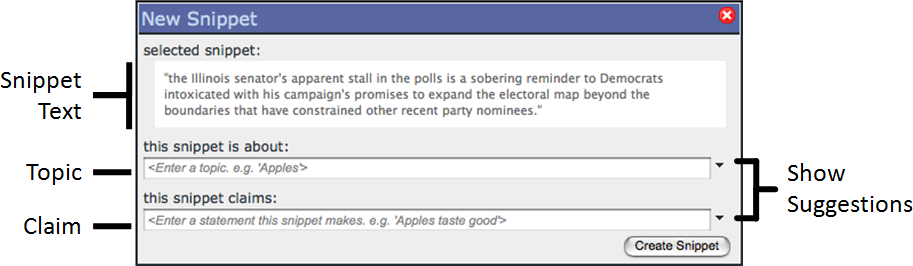
\includegraphics[width=8.5cm]{../screenshots/oldsnipcreate_diagram.png}
	\caption{First Prototype Snippet Creation Dialog}
	\label{oldsnippetbox}
\end{figure}

\begin{figure}[t]
\begin{center}
	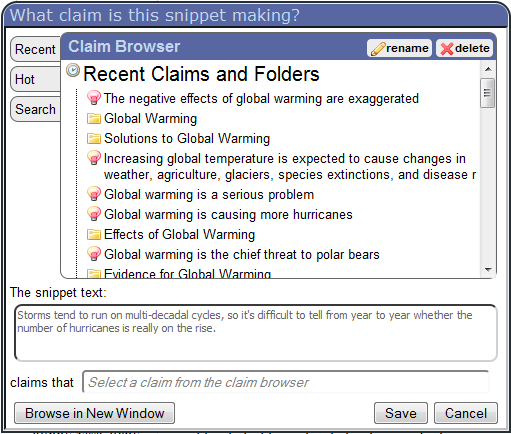
\includegraphics[width=5cm]{../screenshots/newsnip_browseopen.png}
	\caption{Second Prototype Snippet Creation Dialog}
	\label{secondsnippetbox}
\end{center}
\end{figure}

The prototype interfaces required that a user enter a claim for a snippet at the point at which they created the snippet. When the user marked a snippet, Dispute Finder would display a dialog box asking them what claim to associate it with (Figure~\ref{oldsnippetbox} for the first prototype and Figure~\ref{secondsnippetbox} for the second prototype). There turned out to be several problems with this approach:

Users would often encounter a snippet that could be interpreted as making several interesting claims and were confused by the need to pick only one claim. Some users dealt with this by writing a compound claim such as ``Global warming will cause X and Y'', while other users marked several overlapping snippets making different claims. In the final interface one can associate a snippet with several claims.

Some users wanted to associate a snippet with a topic but without associating it with a specific claim. For example, they might find the text of an important speech, or the results of a sporting event. While they might want to use this as evidence for a claim in the future, they didn't yet know what that claim might be. In the final interface one can choose to associate a snippet with a topic.

Some users seemed to be deterred from marking interesting snippets by the mental effort required to choose an appropriate claim. In several cases, we saw a user pause to decide whether an interesting snippet was worth marking up. Similarly, some users seemed to find it difficult to decide what the right claim to use for a snippet was, since they had not yet decided how they wanted to structure their argument, or even if this was a topic they wanted to argue about. The final interface does not require a user to associate a snippet with a claim at the time they create the snippet. Instead a user can mark snippets with minimal effort and then later search through their snippets to find evidence for particular claims.

Several users expressed confusion about how specific the claim made by a snippet should be, or when they should pick an existing claim rather than create a new one. For example, if a snippet says ``Global temperatures will rise by X degrees by 2050'' then is that making the claim ``Global temperatures will rise'', or should the claim include the extra information? In the final interface, users are expected to only create a claim when they have several snippets that support or oppose the same claim. This makes it easier to know how broad the claim should be as the user knows how much information is shared by claims.

Since a user was required to enter a claim whenever they created a snippet, there was an incentive for the user to enter a claim as quickly as possible so they could make the dialog go away. 
Several users created a new claim that was equivalent to a claim that already existed, and several users repeatedly created a claim that had the exact same text as the snippet. The final interface reduces this problem by not requiring a user to associate a claim with a snippet until they decide that this is something that they want to do, and have a particular disputed claim in mind.

\todo{Need to do some kind of evaluation to show that the new interface solves these problems}


\subsubsection{Choosing what to mark as a snippet}

Users would frequently mark the first paragraph of an article as a snippet. This paragraph would frequently summarize the arguments made in the rest of the document document and often made an important claim that other claims in the document supported or provided context for. 

Several users wanted to mark up a table or an image as a snippet. This is valid behavior -- a table or image is often useful evidence for a claim; however it is not currently supported by Dispute Finder. In future versions of Dispute Finder we intend to support this behavior.


\subsubsection{Connecting Claims}

Several participants expressed a desire to connect related claims during their session. 

Some users marked one claim as supporting another when it would have been more logically correct to mark them both as supporting a third claim that needed to be created. For example ``Global warming is causing more hurricanes'' does not support ``Global warming is causing rising sea levels'', but both support ``Global warming is causing problems''. Users realized that the claims were related, but were not sure how best to connect them. It is possible that creating logically correct claim structures may be too difficult for some people (see Isenmann and Reuter~\cite{Isenmann1997}). We believe that this problem can be addressed to some extent though voting by other users who recognize that a claim does not provide useful evidence. 

Some users were confused by claims that had a ``because'' relationship rather than a ``supports'' or ``opposes'' relationship. For example ``America did not sign the Kyoto Protocol'' {\it because} ``Signing Kyoto would harm the US economy''. Similarly, many users expressed a desire to mark claims as being related without supporting or opposing each other. For example ``America did not sign the Kyoto Protocol'' {\it  relates-to} ``America was right to not sign the Kyoto Protocol''. In the final interface we introduced a ``relates-to'' link type to allow users to connect claims that they thought should be related but which didn't confirm to a simple pro/con relationship. 

Several users got confused by claims that referred to similar events at different points in time. 
For example, one participant in the first study marked two claims as opposing each other when each was true at the time that it was written. This is a particular problem when talking about breaking news events, where the facts can change fast. If Dispute Finder is to be effective for describing such events then it will need to have better support associating times with claims and snippets.

Several users expressed an interest in being able to mark a claim as disputed without having to find opposing evidence. One user said that opposing a claim required ``too many clicks'' and they wanted to be able to just vote against a claim without having to say why or find evidence. In the future we are planning to allow users to say what claims they personally believe are true or false and see what claims their friends agreed or disagreed with.

\begin{figure}[tb]
	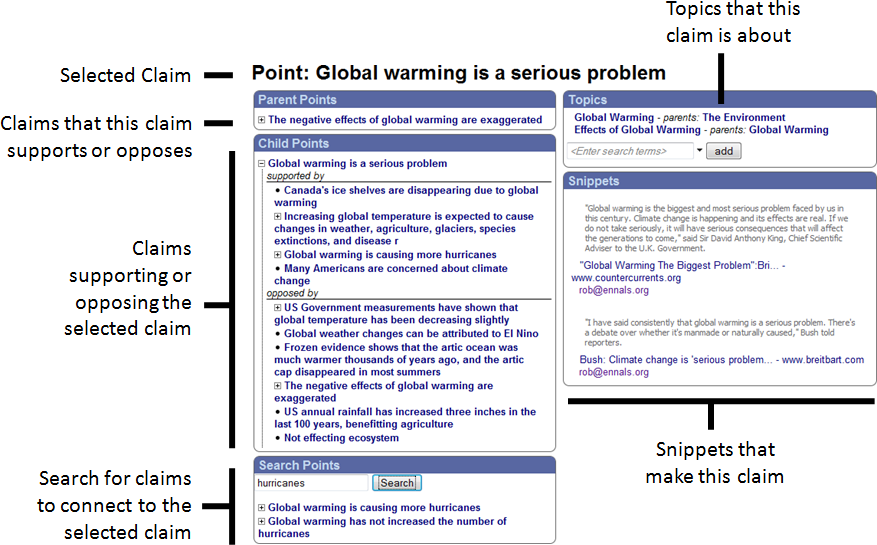
\includegraphics[width=8cm]{../screenshots/oldpoint_diagram.png}
	\caption{First Prototype Claim Browser}
	\label{oldbrowser}
\end{figure}

\begin{figure}[tb]
\begin{center}
	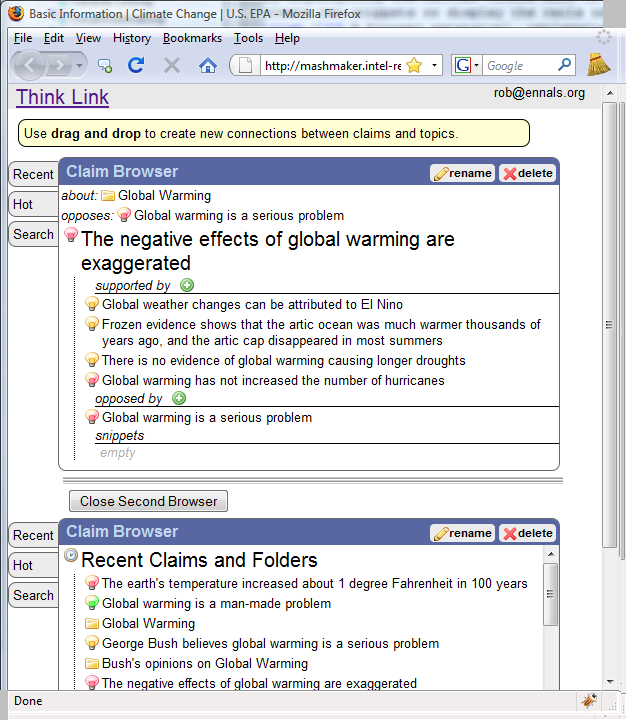
\includegraphics[width=5.5cm]{../screenshots/claimbrowse.png}
	\caption{Second Prototype Claim Browser}
	\label{secondbrowser}
\end{center}
\end{figure}

The prototype versions of Dispute Finder used a drag-and-drop interface to allow a user to create links between claims. In the first interface (Figure~\ref{oldbrowser}) a user could use a search box to find others' claims and then drag them into appropriate positions in the argument graph. The second interface (Figure~\ref{secondbrowser}) followed a file-manager metaphor, providing two identical browser windows that a user could drag and drop claims between. 
In both cases, we found that users would often not realize they could use drag and drop to organize claims, even when we added a prominent information message at the top of the display (Figure~\ref{secondbrowser}). We believe that part of the problem was that users are not used to using drag-and-drop in a web interface, and the rendering of a claim did not have any visual clue to suggest that they could use drag and drop to create connections. In the final interface we resolved this issue by moving to a ``click to link'' interface and having the connection actions (``add claim'' etc) prominently visible.

\section{Conclusions and Future Work}

We have introduced the idea of highlighting disputed claims and connecting them to sources that give alternative points of view. We have created an interface that makes it easy for users to explore evidence that supports or opposes a claim, and makes it easy for users to gather and connect new snippets. 

At present Dispute Finder relies on users to mark up snippets and connect them to claims. In the future we plan to explore using natural language and machine learning techniques to assist in this process. Our plan is to allow a user to request that Dispute Finder search the web to find potential snippets that make a claim that they disagree with, and then quickly select which of these are indeed making the claim.

Dispute Finder is designed to be used as a social tool in which large numbers of people collaborate to find large numbers of claims and snippets about interesting topics. Since our graph and user base are currently small, we have not yet evaluated how Dispute Finder works when data sets are huge, many users are concurrently editing data, and some users are malicious.

We hope that Dispute Finder will make it easier for people to be informed about the world and be exposed to alternative points of view that they might not otherwise be exposed to.

\section{Acknowledgments}

Acknowledgements omitted for blind submission. Dispute Finder uses icons from the free FamFamFam Silk\footnote{http://famfamfam.com} collection.


\todo{Sort out bad references}
\bibliography{refs}

\end{document}



